% This document is based on a template created by Ted Pavlic (http://www.tedpavlic.com)


%----------------------------------------------------------------------------------------
%	PACKAGES AND OTHER DOCUMENT CONFIGURATIONS
%----------------------------------------------------------------------------------------

\documentclass{article}

\usepackage{fancyhdr} % Required for custom headers
\usepackage{lastpage} % Required to determine the last page for the footer
\usepackage{extramarks} % Required for headers and footers
\usepackage[usenames,dvipsnames]{color} % Required for custom colors
\usepackage{graphicx} % Required to insert images
\usepackage{subcaption}
\usepackage{listings} % Required for insertion of code
\usepackage{courier} % Required for the courier font
%\usepackage{lipsum} % Used for inserting dummy 'Lorem ipsum' text into the template
\usepackage{amsmath,siunitx,physics,amssymb}
\usepackage{cleveref}
\usepackage{placeins}
\usepackage{enumitem}
\usepackage{minted,xcolor}

% Margins
\topmargin=-0.45in
\evensidemargin=0in
\oddsidemargin=0in
\textwidth=6.5in
\textheight=9.0in
\headsep=0.25in

\linespread{1.1} % Line spacing

% Set up the header and footer
\pagestyle{fancy}
\lhead{\hmwkAuthorName} % Top left header
\chead{\hmwkClass\ (\hmwkClassTime): \hmwkTitle} % Top center head
%\rhead{\firstxmark} % Top right header
\lfoot{\lastxmark} % Bottom left footer
\cfoot{} % Bottom center footer
\rfoot{Page\ \thepage\ of\ \protect\pageref{LastPage}} % Bottom right footer
\renewcommand\headrulewidth{0.4pt} % Size of the header rule
\renewcommand\footrulewidth{0.4pt} % Size of the footer rule

%\setlength\parindent{0pt} % Removes all indentation from paragraphs

%----------------------------------------------------------------------------------------
%	DOCUMENT STRUCTURE COMMANDS
%	Skip this unless you know what you're doing
%----------------------------------------------------------------------------------------

% Header and footer for when a page split occurs within a problem environment
\newcommand{\enterproblemHeader}[1]{
%\nobreak\extramarks{#1}{#1 continued on next page\ldots}\nobreak
%\nobreak\extramarks{#1 (continued)}{#1 continued on next page\ldots}\nobreak
}

% Header and footer for when a page split occurs between problem environments
\newcommand{\exitproblemHeader}[1]{
%\nobreak\extramarks{#1 (continued)}{#1 continued on next page\ldots}\nobreak
%\nobreak\extramarks{#1}{}\nobreak
}

\setcounter{secnumdepth}{0} % Removes default section numbers
\newcounter{problem} % Creates a counter to keep track of the number of problems
\setcounter{problem}{-1}

\newcommand{\problemName}{}
\newenvironment{problem}[1][Part \theproblem]{ % Makes a new environment called problem which takes 1 argument (custom name) but the default is "problem #"
	\stepcounter{problem} % Increase counter for number of problems
	\renewcommand{\problemName}{#1} % Assign \problemName the name of the problem
	\section{\problemName} % Make a section in the document with the custom problem count
	\enterproblemHeader{\problemName} % Header and footer within the environment
}{
	\exitproblemHeader{\problemName} % Header and footer after the environment
}

\newcommand{\problemAnswer}[1]{ % Defines the problem answer command with the content as the only argument
	\noindent\framebox[\columnwidth][c]{\begin{minipage}{0.98\columnwidth}#1\end{minipage}} % Makes the box around the problem answer and puts the content inside
}

\newcounter{subproblem}[problem]
\newcommand{\subproblemName}{}
\newenvironment{subproblem}[1][\theproblem~(\alph{subproblem})]{ % New environment for sections within  problems, takes 1 argument - the name of the section
	\stepcounter{subproblem}
	\renewcommand{\subproblemName}{#1} % Assign \problemName the name of the problem
	\subsection{\subproblemName} % Make a section in the document with the custom problem count
	\enterproblemHeader{\subproblemName} % Header and footer within the environment
}{
	\enterproblemHeader{\problemName} % Header and footer after the environment
}

\newcommand{\numberthis}{\addtocounter{equation}{1}\tag{\theequation}}

%----------------------------------------------------------------------------------------
%	NAME AND CLASS SECTION
%----------------------------------------------------------------------------------------

\newcommand{\hmwkTitle}{Assignment\ \#$1$} % Assignment title
\newcommand{\hmwkDueDate}{Friday,\ January\ 29,\ 2018} % Due date
\newcommand{\hmwkClass}{CSC411} % Course/class
\newcommand{\hmwkClassTime}{L2001} % Class/lecture time
\newcommand{\hmwkAuthorName}{Lukas Zhornyak} % Your name

%----------------------------------------------------------------------------------------
%	TITLE PAGE
%----------------------------------------------------------------------------------------

\title{
	\vspace{2in}
	\textmd{\textbf{\hmwkClass:\ \hmwkTitle}}\\
	\normalsize\vspace{0.1in}\small{Due\ on\ \hmwkDueDate}\\
	\vspace{0.1in}
	\vspace{3in}
}

\author{\textbf{\hmwkAuthorName}}
%\date{} % Insert date here if you want it to appear below your name

%----------------------------------------------------------------------------------------

\begin{document}

\maketitle
\clearpage

%----------------------------------------------------------------------------------------
%	ENVIRONMENT
%----------------------------------------------------------------------------------------

\begin{problem}[Environment]	
	Parts 1-6 were created with Python 2.7.14 with numpy 1.14.0, scipy 1.0.0, scikit-image 0.13.1, and matplotlib 2.1.1, as well as all associated dependencies. Parts 8-10 were created with Python 3.6.4 with numpy 1.14.1, scipy 1.0.0, scikit-image 0.13.1, and matplotlib 2.1.2, pytorch 0.3.0, torchvision 0.2.0, as well as all associated dependencies.
\end{problem}
\clearpage

%----------------------------------------------------------------------------------------
%	PART 1
%----------------------------------------------------------------------------------------
\FloatBarrier
\begin{problem}
	The dataset, provided in assignment, is already split into training and validation sets. About six thousand images are provided in the training set for each digit (ranging from 5421 to 6742) while about one thousand images are provided in the testing set (ranging from 892 to 1135), for a total of about seven thousand images in the combined set for each digit. In total, there are sixty thousand training images and ten thousand testing images. Ten randomly selected images from the combined training and testing sets are shown in \cref{digits}.
	
	Due to the way the images are selected and displayed, any images selected that were from the validation set would be shown on the second row and right side of the set of images for each digit shown in \cref{digits}. As cab be seen, there does not seem to be any major systematic variation in the images from the validation set compared to the images from the training set. This is to be expected and is necessary for the proper training of the classifier.
	
	The images provided are typical of digits written quickly and without specific care to how they appear; in other words, they represent digits how they would likely appear in an arbitrary handwritten sample. The digits do not seem specifically drawn for clarity. While the positioning and the size remain approximately consistent between digits, the geometry of the digits is not completely consistent. For example, some two's are written with a loop while other's are not. Additionally, the slant and stroke thickness of the digit varies considerably.
	
	\begin{figure}[bh]
		\begin{subfigure}{\linewidth}
			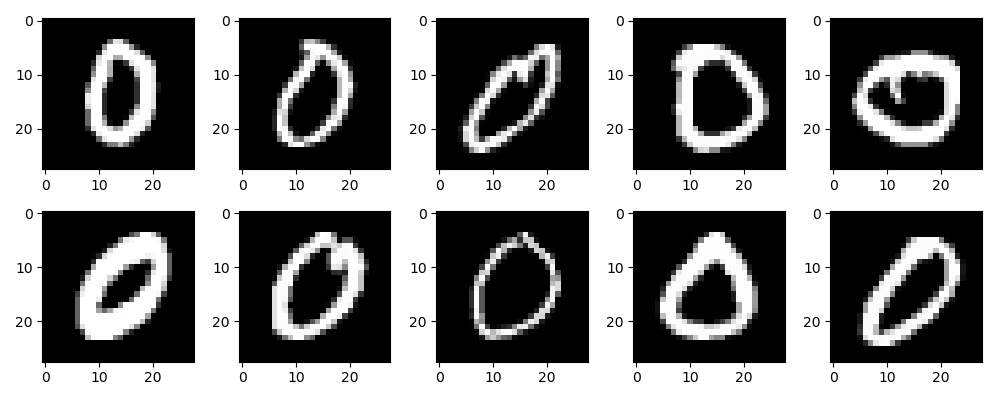
\includegraphics[width=\linewidth]{sample_digits_0}
		\end{subfigure}
		\caption{Random sample of each digit selected from the complete dataset.}
	\end{figure}
	\begin{figure}\ContinuedFloat
		\begin{subfigure}{\linewidth}
			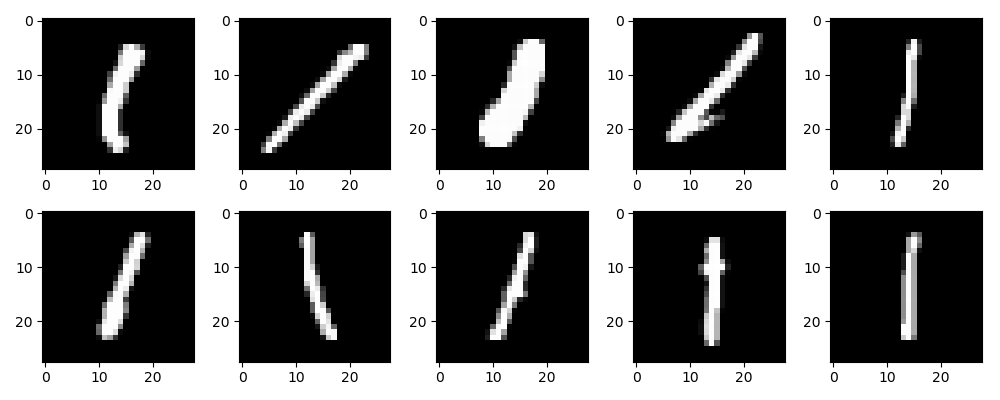
\includegraphics[width=\linewidth]{sample_digits_1}
		\end{subfigure}
		\begin{subfigure}{\linewidth}
			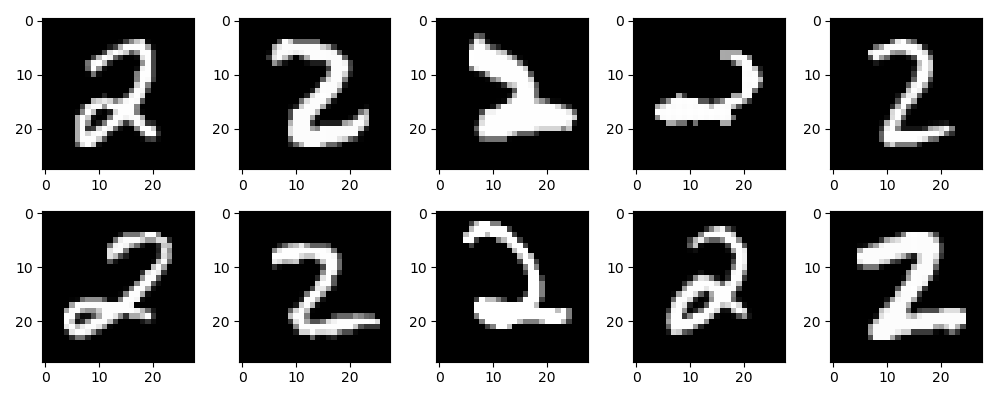
\includegraphics[width=\linewidth]{sample_digits_2}
		\end{subfigure}
		\begin{subfigure}{\linewidth}
			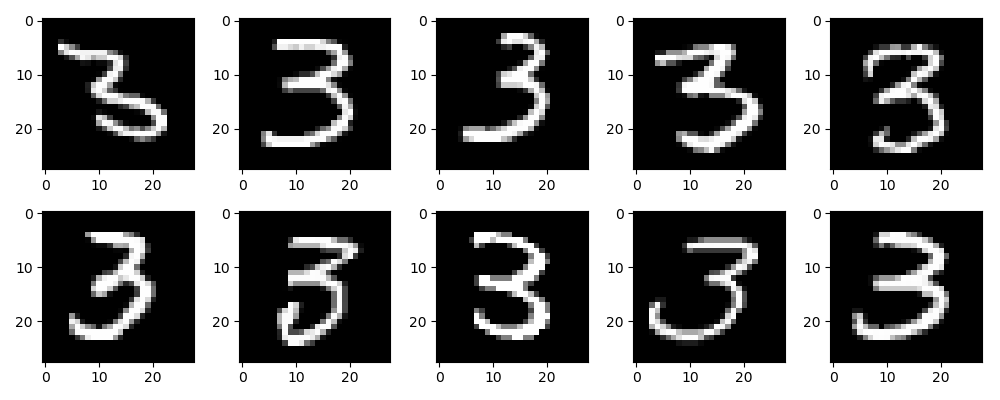
\includegraphics[width=\linewidth]{sample_digits_3}
		\end{subfigure}
		\caption{\textit{Cont.} Random sample of each digit selected from the complete dataset.}
	\end{figure}
	\begin{figure}\ContinuedFloat
		\begin{subfigure}{\linewidth}
			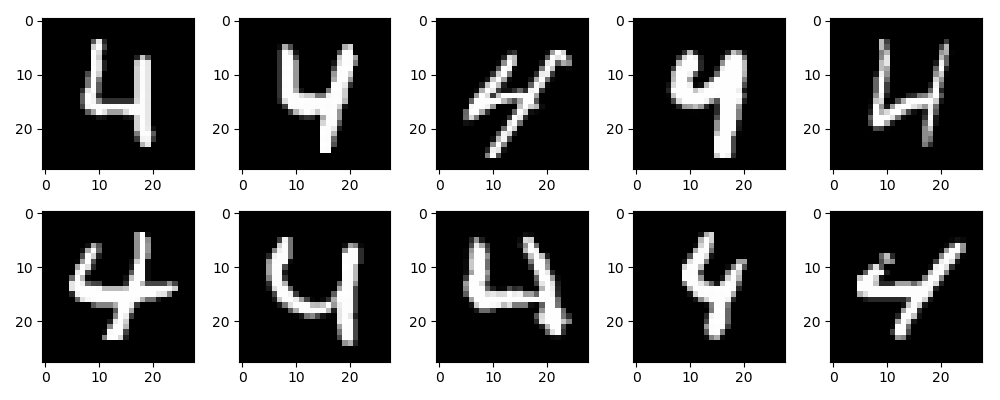
\includegraphics[width=\linewidth]{sample_digits_4}
		\end{subfigure}
		\begin{subfigure}{\linewidth}
			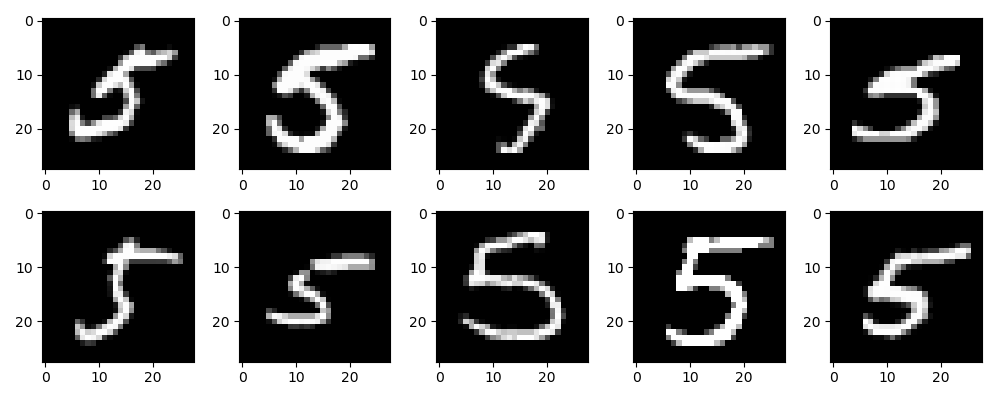
\includegraphics[width=\linewidth]{sample_digits_5}
		\end{subfigure}
		\begin{subfigure}{\linewidth}
			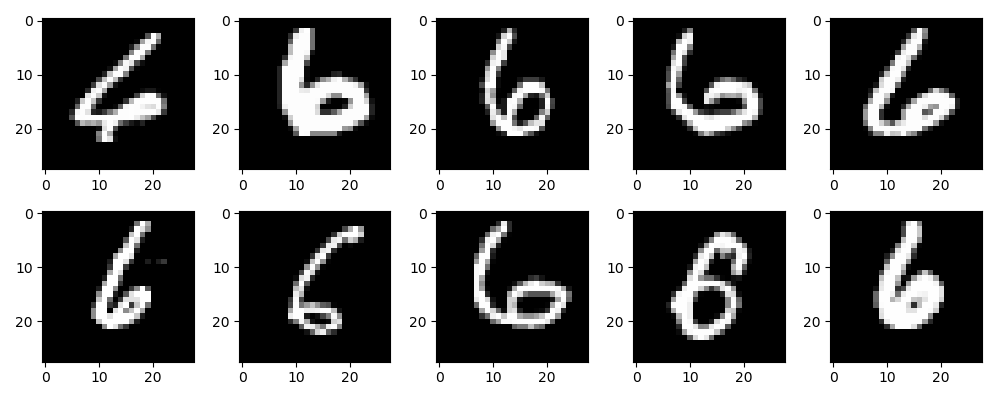
\includegraphics[width=\linewidth]{sample_digits_6}
		\end{subfigure}
		\caption{\textit{Cont.} Random sample of each digit selected from the complete dataset.}
	\end{figure}
	\begin{figure}\ContinuedFloat
		\begin{subfigure}{\linewidth}
			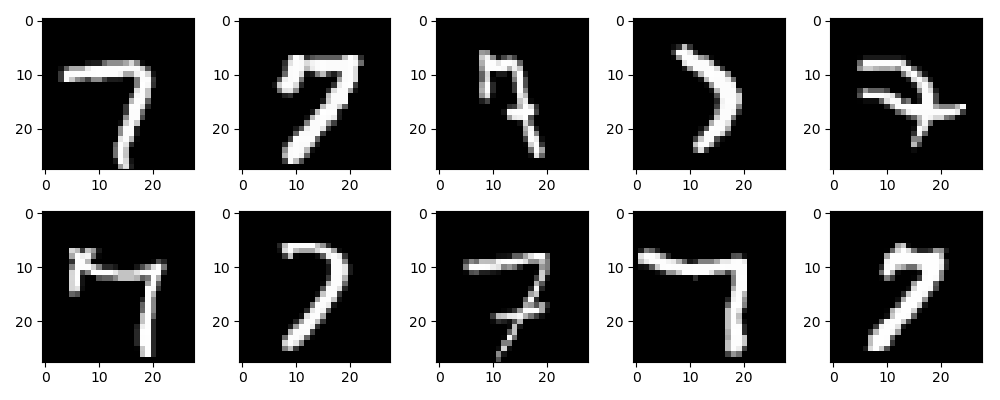
\includegraphics[width=\linewidth]{sample_digits_7}
		\end{subfigure}
		\begin{subfigure}{\linewidth}
			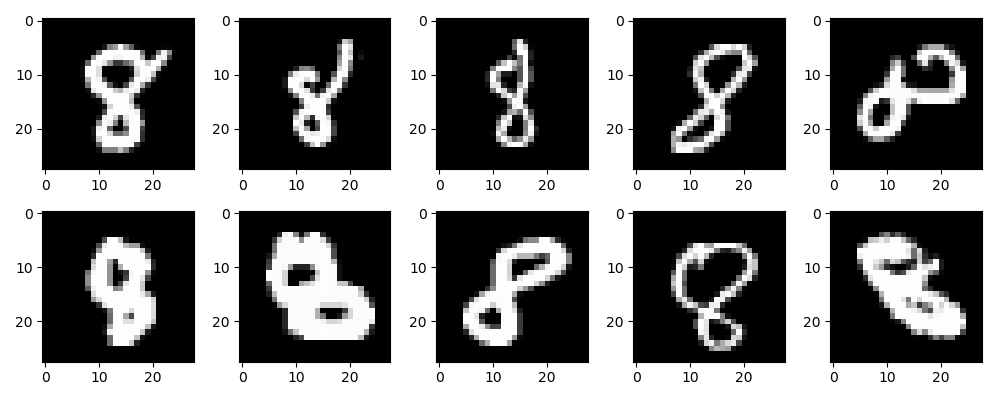
\includegraphics[width=\linewidth]{sample_digits_8}
		\end{subfigure}
		\begin{subfigure}{\linewidth}
			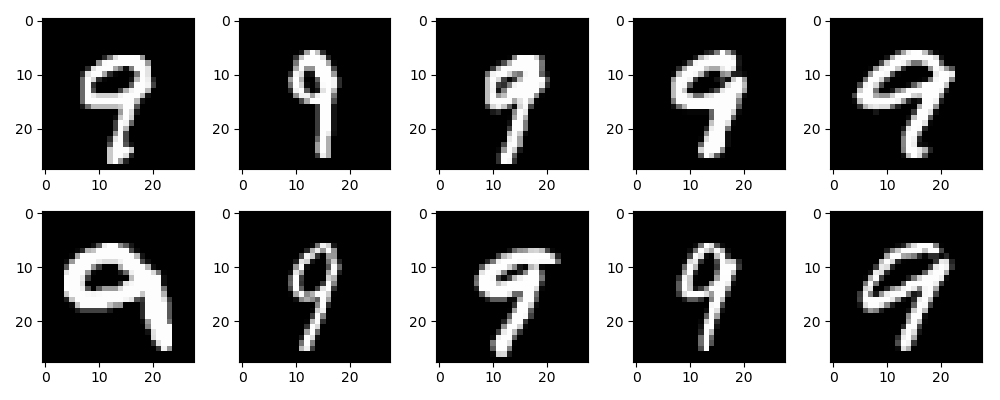
\includegraphics[width=\linewidth]{sample_digits_9}
		\end{subfigure}
		\caption{\textit{Cont.} Random sample of each digit selected from the complete dataset.}
		\label{digits}
	\end{figure}
\end{problem}
\clearpage

%----------------------------------------------------------------------------------------
%	PART 2
%----------------------------------------------------------------------------------------

\begin{problem}
	With the provided softmax function:
	
	\begin{minted}[mathescape, linenos, numbersep=5pt, gobble=2, frame=lines, framesep=2mm, tabsize=4, breaklines]{python}
		def basic_network(W, x, b):
			return softmax(np.dot(W, x) + b)
	\end{minted}	
	
\end{problem}
\clearpage

%----------------------------------------------------------------------------------------
%	PART 3
%----------------------------------------------------------------------------------------

\begin{problem}
\begin{subproblem}
	We want to find \(\pdv{C}{\omega_{ij}}\) the derivative of the weight \(\omega_{ij}\) associated with the connection from the \(j\)-th input node \(x_j\) to the \(i\)-th output node \(o_i\), before the softmax.  The derivative can thus be expanded via the chain rule as
	\begin{equation}\label{q3.1}
		\pdv{C}{\omega_{ij}} = \sum_k\pdv{C}{o^{(k)}_i}\pdv{o^{(k)}_i}{\omega_{ij}}
	\end{equation} 
	Where the superscript denotes the \(k\)-th member of the set. Since \(\omega_{ij}\) only influences the value of \(o_i\), the derivatives of other output nodes with respect to \(\omega_{ij}\) will be zero and are thus not included in the above equation. Each of these derivatives can now be found separately. The second can be found trivially since we assume an identity activation function, giving. 
	\begin{equation} \label{q3.2}
		\pdv{o^{(k)}_i}{\omega_{ij}} = x^{(k)}_j
	\end{equation}
	Examining first part of the derivative of the cost function:
	\begin{align*}
		C &= -\sum_k \sum_\ell y^{(k)}_\ell \log(p^{(k)}_\ell) \\
		\Rightarrow\quad \pdv{C}{o^{(k)}_i} &= -\sum_k \sum_\ell y^{(k)}_\ell \pdv{\log(p^{(k)}_\ell)}{o^{(k)}_i}\numberthis\label{q3.3}
	\end{align*}
	Where \(p\) is the output after the softmax and \(y\) is the actual label. Dropping the superscript for clarity,
	\begin{align*}
		\log(p_\ell) &= \log(\frac{\exp(o_\ell)}{\sum_m \exp(o_m)}) \\
		&= o_\ell - \log(\sum_m \exp(o_m)) \\
		\Rightarrow\quad \pdv{\log(p_\ell)}{o_i} &= \pdv{o_\ell}{o_i} - \frac{\exp(o_i)}{\sum_m \exp(o_m)} \\
		&= \begin{cases}
			1 - p_i & i = j \\
			-p & i \ne j
		\end{cases} \numberthis\label{q3.4}
	\end{align*}
	Subbing \cref{q3.4} into \cref{q3.3} thus produces:
	\begin{align*}
		\pdv{C}{o^{(k)}_i} &= \sum_k \qty(\qty(\sum_\ell y^{(k)}_\ell p^{(k)}_i) - y^{(k)}_i) \\
		&= \sum_k \qty(p^{(k)}_i - y^{(k)}_i) \numberthis \label{q3.5}
	\end{align*}
	Where one-hot encoding was assumed, resulting in \(\sum_\ell y^{(k)}_\ell = 1\). Substituting \cref{q3.2,q3.5} into \cref{q3.1} produces the complete expression for the gradient.
	\begin{equation}\label{q3s}
		\pdv{C}{\omega_{ij}} = \sum_k \qty(p^{(k)}_i - y^{(k)}_i) x^{(k)}_j
	\end{equation}
	This can also be expressed in vector form as
	\begin{equation}\label{q3v}
		\pdv{C}{W} = \sum_k \qty(p^{(k)} - y^{(k)}) \qty(x^{(k)})^\mathsf{T}
	\end{equation}
\end{subproblem}
\begin{subproblem}
	The code used to compute the gradient with respect to both the weights and the biases is shown below. Note that all quantities are transposed compared to the formula shown in \cref{q3v}, hence the small differences.
	\begin{minted}[mathescape, linenos, numbersep=5pt, gobble=2, frame=lines, framesep=2mm, tabsize=4, breaklines]{python}
		def basic_gradient(W, x, b, y):
			p = basic_network(W, x, b)
			return np.dot(x.T, p - y), np.sum(p - y, 0)
	\end{minted}
\end{subproblem}
\end{problem}
\clearpage

%----------------------------------------------------------------------------------------
%	PART 4
%----------------------------------------------------------------------------------------

\FloatBarrier
\begin{problem}
	The learning curve after ten thousand generations of stochastic gradient descent is shown in \cref{fig:learn curve} and a visualization of the resultant weights is shown in \cref{fig:digit vis}. For this optimization, the training sets for each individual digit were combined into one large set and an additional array with the corresponding labels was created. 
	
	The initial weights were initialized using Xavier Initialization. Each weight was thus sampled from a normal distribution centred at zero and with a variance of \(\frac{1}{140}\), corresponding to \(\frac{2}{n_{in} + n_{out}}\). The weights were trained on mini batches of size 1000, selected through trial and error as a compromise between speed and stability The learning rate was selected as \num{1e-5} as this was the largest rate (to an order of magnitude) that did not result in the runaway growth of the weights. 

\begin{figure}
	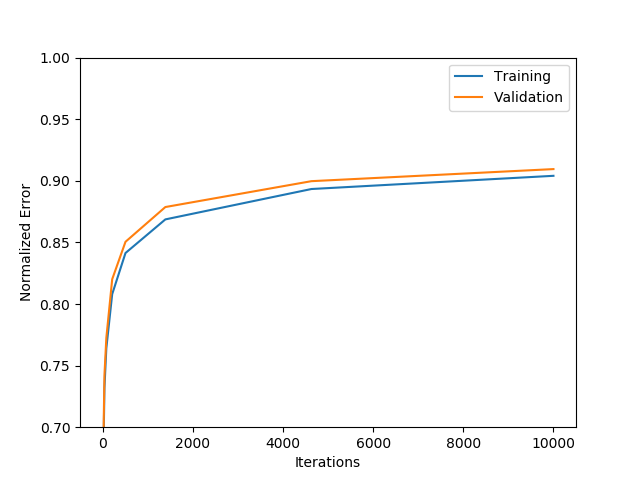
\includegraphics[width=\linewidth]{learning_rate}
	\caption{Performance on the provided training and verification sets after ten thousand generations of training on the training set using stochastic gradient descent. Note that "Normalized Error" should read accuracy.}
	\label{fig:learn curve}
\end{figure}

\begin{figure}
	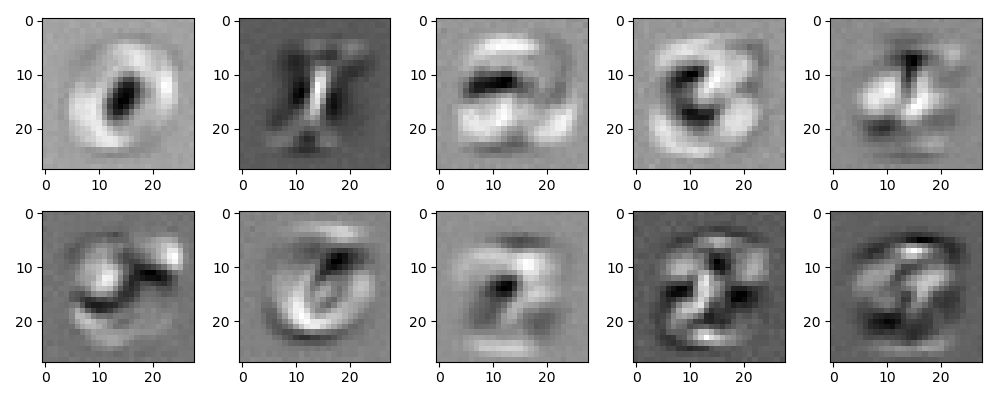
\includegraphics[width=\linewidth]{digit_visualization}
	\caption{Visualization of the weights going into each output node after stochastic gradient descent. Visualization is constructed so that the location of each weight corresponds to the location of the input node that it corresponds to. Note the resemblance to generic numerals.}
	\label{fig:digit vis}
\end{figure}

\end{problem}
\clearpage

%----------------------------------------------------------------------------------------
%	PART 5
%----------------------------------------------------------------------------------------

\begin{problem}
	The function used to perform gradient descent with momentum is given below. Note that several lines related to recording and plotting the error and progress are removed for brevities sake. The resulting learning curve and weights after \num{10000} (the same as in problem 4) are shown in \cref{fig:digit vis momentum,fig:learn curve momentum}, respectively.
	
	\begin{minted}[mathescape, linenos, numbersep=5pt, gobble=2, frame=lines, framesep=2mm, tabsize=4, breaklines]{python}
		def gradient_descent(W, x, b, y, xv, yv, learning_rate=1e-5, epsilon=1e-8, max_iter=1000, momentum=0.9, save_file=None):
			W = W.copy()  # ensure that passed in value not changed
			b = b.copy()
			last = np.zeros_like(W)
			i = 0
			dW, db = 0, 0
			while np.linalg.norm(W - last) > epsilon and i < max_iter:
				last = W.copy()
				dW_n, db_n = basic_gradient(W, x, b, y)
				dW = dW * momentum - dW_n * learning_rate
				db = db * momentum - db_n * learning_rate
				W += dW
				b += db
				i += 1
			return W, b
	\end{minted}
	
	\begin{figure}
		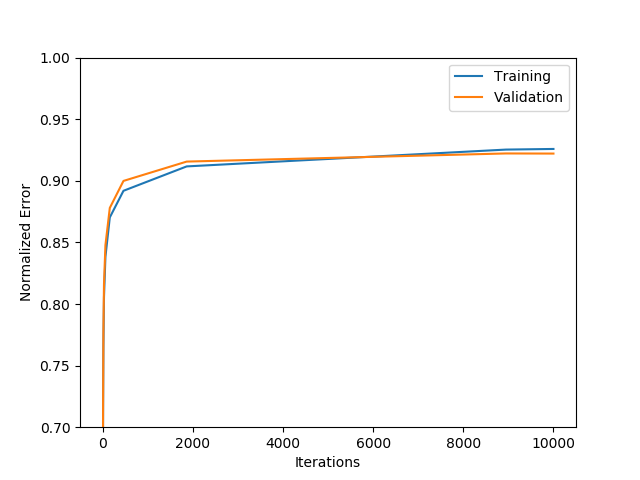
\includegraphics[width=\linewidth]{learning_rate_momentum}
		\caption{Performance on the provided training and verification sets after ten thousand generations of training on the training set using stochastic gradient descent with momentum.}
		\label{fig:learn curve momentum}
	\end{figure}
	
	\begin{figure}
		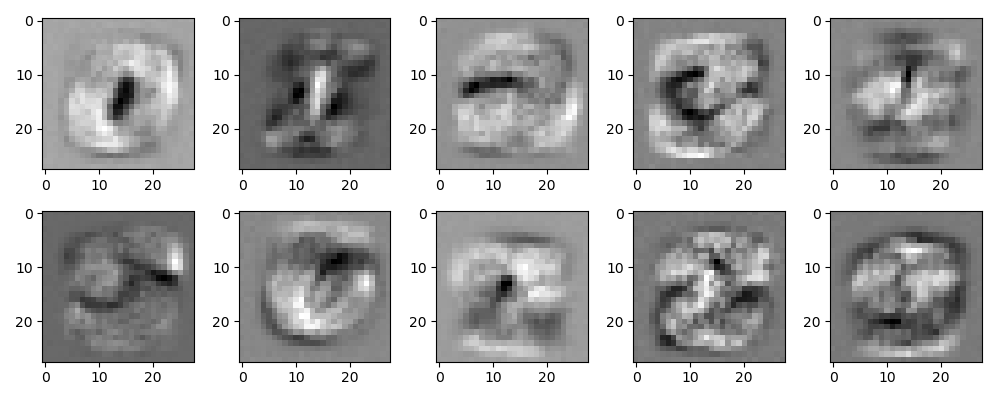
\includegraphics[width=\linewidth]{digit_visualization_momentum}
		\caption{Visualization of the weights going into each output node after stochastic gradient descent with momentum. Visualization is constructed so that the location of each weight corresponds to the location of the input node that it corresponds to. Note the resemblance to generic numerals. Note that "Normalized Error" should read "Accuracy".}
		\label{fig:digit vis momentum}
	\end{figure}
\end{problem}
\clearpage

%----------------------------------------------------------------------------------------
%	PART 6
%----------------------------------------------------------------------------------------

\FloatBarrier
\begin{problem}
	The contour plot and trajectories of the two weights are shown in \cref{fig:low mom}. This figure shows that using momentum properly will allow for faster convergence than without. Specifically, the use of momentum significantly reduces the oscillations associated with going down a valley as one bounces from one wall to another while at the same time increases the rate that one moves down the valley. This is because the momentum term, in a sense, pushes the gradient descent to keep moving in the same direction that it was going. This compounds the effects of gradients pointing in similar direction while reducing the effects of gradients pointing in opposite directions. 
	
	To produce these visualization, the pixels located at (13, 13) in the "0" weights and the "1" weights were chosen as \(w_1\) and \(w_2\), respectively. A pixel near the centre was chosen as the weights associated with it would be necessary to distinguish numbers, producing large enough gradients. Additionally, to show the effects of momentum a contour that is considerably narrower one way than the other is also desirable as such situations are where the momentum term really shows its effect. A learning rate of \num{6e-3} was selected through trial and error and used for both types of gradient descent to highlight the differences of just the momentum term.
	
	\Cref{fig:high mom} shows an identical figure to that shown in \cref{fig:low mom}, except the momentum has been set to 0.8 rather than 0.25. This higher momentum means that the gradient descent overshoots the actual minimum and spends longer circling around the minimum. This happens because the large momentum term means that the descent is less able to react to sharp changes in the slope of the gradient, the momentum term acting as a form of exponential smoothing.
	
	\begin{figure}
		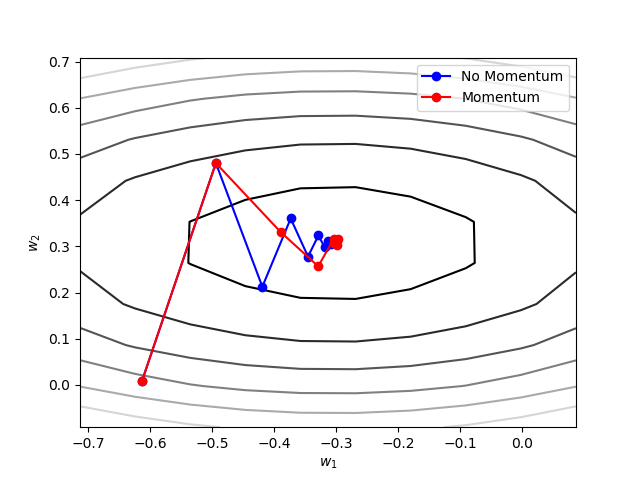
\includegraphics[width=\linewidth]{mom_vs_no_mom}
		\caption{Visualization of the path of the gradient descent without momentum and with a momentum of 0.25.}
		\label{fig:low mom}
	\end{figure}
	\begin{figure}
		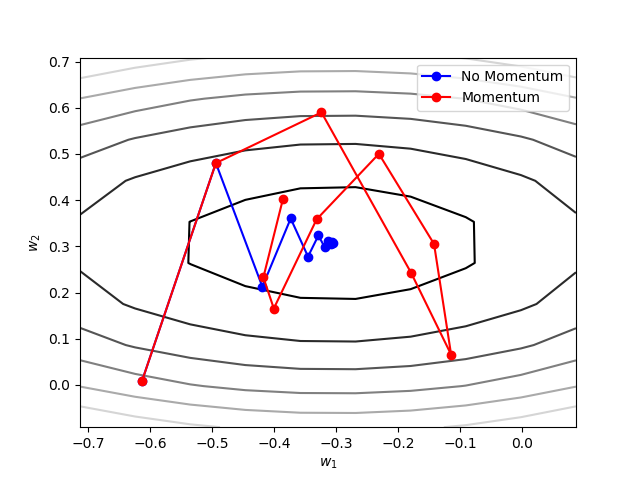
\includegraphics[width=\linewidth]{mom_vs_no_mom_2}
		\caption{Visualization of the path of the gradient descent without momentum and with a momentum of 0.8.}
		\label{fig:high mom}
	\end{figure}
\end{problem}
\clearpage

%----------------------------------------------------------------------------------------
%	PART 7
%----------------------------------------------------------------------------------------

\begin{problem}
	Let \(y_i^{(\ell)}\) be the \(i\)-th node in the \(ell\)-th layer, where \(y^{(1)}\) is the input layer and \(y^{(N)}\) is the output layer for a total of \(N\) layers with \(K\) nodes in each layer. Let \(\omega_{ij}^{(\ell)}\) be the weight associated with the connection of node \(j\) in the layer \(\ell\) to node \(i\) of the layer \(\ell + 1\). Then, the formula expressing one layer in terms of the previous, for \(\ell  > 1\) and assuming no biases, can be expressed as
	\begin{equation*}
		y_i^{(\ell)} = a\qty(\sum_{j=1}^K \omega_{ij}^{(\ell - 1)} y_i^{(\ell - 1)})
	\end{equation*}
	where \(a\) is the activate function. The derivative of \(y_i^{(\ell)}\) with respect to a weight connecting a node in the previous layer to it can thus be expressed as
	\begin{equation}\label{eq:dw}
		\pdv{y_i^{(\ell)}}{\omega_{im}^{(\ell - 1)}} = a'\qty(y_i^{(\ell)})y_m^{(\ell)}
	\end{equation}
	Similarly, the derivative of \(y_i^{(\ell)}\) with respect to the node \(m\) in layer \(p\), \(p < \ell\), can be expressed as
	\begin{equation}\label{eq:dy}
		\pdv{y_i^{(\ell)}}{y_m^{(p)}} = a'\qty(y_i^{(\ell)})\qty(\sum_{j=1}^K \omega_{ij}^{(\ell - 1)} \pdv{y_j^{(\ell - 1)}}{y_m^{(p)}})
	\end{equation}
	requiring the computation of an additional \(K\) derivatives.
	
	Assume that basic multiplication takes time \(t_m\), addition takes time \(t_+\), find \(a'(y)\) for some y takes time \(t_a\), and finding the derivative of the cost function \(C\) with respect to one of the output nodes takes time \(t_C\). Additionally, assume all values \(y_i^{(\ell)}\), produced as a result of forward propagation, are cached. Then, the cost of \cref{eq:dw} can be expressed as
	\begin{equation*}
		T\qty(\pdv{y_i^{(\ell)}}{\omega_{im}^{(\ell - 1)}}) = t_a + t_m
	\end{equation*}
	while the cost of \cref{eq:dy} can be expressed as, assuming \(K \gg 1\) and \(N \gg 1\),
	\begin{align*}
		T\qty(\pdv{y_i^{(\ell)}}{y_m^{(p)}}) &= t_a + t_m + (K-1)t_+ + \sum_{j=1}^K \qty(t_m + T\qty(\pdv{y_j^{(\ell - 1)}}{y_m^{(p)}}))\\
		&= t_a + (K+1)t_m + (K-1)t_+ + \sum_{j=1}^K T\qty(\pdv{y_j^{(\ell - 1)}}{y_m^{(p)}}) \\
		&= \sum_{q = 1}^{\ell - p} K^{q - 1}\qty(t_a + (K+1)t_m + (K-1)t_+) \\
		&= \qty(t_a + (K+1)t_m + (K-1)t_+) \frac{1 - K^{(\ell - p)}}{1 - K} \\
		&= O\qty(K^{\ell - p})
	\end{align*}
	Combining all this together and assuming that \(N > p > 0\), the time taken for the derivative of the cost function with respect to a single weight is
	\begin{align*}
		T\qty(\pdv{C}{\omega_{nm}^{(p)}}) &= T\qty(\sum_{i=1}^{K}\pdv{C}{y_i^{(N)}}\pdv{y_i^{(N)}}{y_n^{(p+1)}}\pdv{y_n^{(p+1)}}{\omega_{nm}^{(p)}}) \\
		&= K\qty(t_c + t_a + 3 t_m + O\qty(K^{N - p - 1})) + (K - 1)t_+ \\
		&= O\qty(K^{N - p})
	\end{align*}
	The total cost to compute the gradients without cached backpropagation is thus
	\begin{align*}
		T\qty(\pdv{C}{W}) &= \sum_{i=1}^{N-1}\sum_{j=1}^K\sum_{n=1}^K O\qty(K^{N - i}) \\
		&= \sum_{i = 1}^{N-1}O\qty(K^{N - i + 2}) \\
		&= O\qty(K^{N+1}\sum_{i = 0}^{N-2}K^{-i}) \\
		&= O\qty(K^{N+1})\numberthis \label{eq:full cost}
	\end{align*}
	
	
	However, through the use of backpropagation and caching, this value can be significantly reduced. First, note that the derivative of the cost function with respect to a given weight can be expressed as
	\begin{align*}
		\pdv{C}{\omega_{nm}^{(p)}} &= \sum_{i=1}^{K}\pdv{C}{y_i^{(p+2)}}\pdv{y_i^{(p+2)}}{y_n^{(p+1)}}\pdv{y_n^{(p+1)}}{\omega_{nm}^{(p)}} \\
		&= \qty(\sum_{i=1}^{K} \pdv{C}{y_i^{(p+2)}} \omega_{in}^{(p+1)}) \pdv{y_n^{(p+1)}}{\omega_{nm}^{(p)}}
	\end{align*}
	if \(p + 1 < N\). If the quantity \(\sum_{i=1}^{K} \pdv{C}{y_i^{(p+2)}} \omega_{in}^{(p+1)} = \pdv{C}{y_n^{(p+1)}}\) is cached, it can then be used to speed up the calculation of the next layer. Thus, the cost to compute an individual gradient (assuming the previous result is cached) reduces to
	\begin{align*}
		T\qty(\pdv{C}{\omega_{nm}^{(p)}}) &= T\qty(\qty(\sum_{i=1}^{K} \pdv{C}{y_i^{(p+2)}} \omega_{in}^{(p+1)}) \pdv{y_n^{(p+1)}}{\omega_{nm}^{(p)}}) \\
		&= t_a + (K+2)t_m + (K-1)t_+ \\
		&= O(K)
	\end{align*}
	while the cost to compute the full gradient is
	\begin{align*}
		T\qty(\pdv{C}{W}) &= \sum_{i=1}^{N-1}\sum_{n=1}^K\sum_{m=1}^K O\qty(K) \\
		&= O(NK^3) \numberthis \label{eq:cached cost}
	\end{align*}
	
	Comparing \cref{eq:full cost,eq:cached cost}, the benefits of using backpropagation are clear. The time to find all the weights individually shows polynomial growth to a large order (\(N + 1\)) with respect to the number of nodes in a layer and \textit{exponential} growth with respect to the number of layers. Meanwhile, backpropagation shows quadratic growth with respect to the number of nodes in a layer and only linear growth with respect to the number of layers. In other words, backpropagation is \(O(K^{N-3}/N)\) times faster than finding the weights individually.
\end{problem}
\clearpage

%----------------------------------------------------------------------------------------
%	PART 8
%----------------------------------------------------------------------------------------

\FloatBarrier
\begin{problem}
	The general structure of the network used takes in a flattened black and white image of some size, gets linearly transformed then has a non linear transfer function applied to reach the hidden layer, then gets linearly transformed again to produce the six outputs the result in one hot encoding. The weights for the network are initialised using Xavier initialization. The images used were downloaded from the internet using the same function as in the last assignment, checking for valid hashes and bounding boxes to ensure that only faces were captured. Unfortunately, not enough Peri Gilpin images were downloaded this way, so the size of the associated sets were scaled down appropriately resulting in 54 training images, 16 validation images, and 16 testing images. The remaining actors were tested with 64 training images, 20 validation images, and 20 testing images.
	
	The hyperparameters varied in this model are the image size, size of the hidden layer, number of epochs, batch size, activation function, and initial learning rate for the optimizer. A grid search was performed on these parameters, with the combination producing the highest accuracy on the validation set selected as the optimal set. The parameters were selected from the following, chosen to represented the likely parameters based on previously conducted trial and error:
	\begin{itemize}[leftmargin=10em]
		\item[Image Size] \(\in \{32, 64\}\)
		\item[Size of Hidden Layer] \(\in \{10, 20, 50\}\)
		\item[Number of Epochs] \(\in \{200, 300, 500\}\)
		\item[Batch Size] \(\in \{20, 50, 100\}\)
		\item[Activation Function] \(\in \{ReLU, LeakyReLU(0.01)\}\)
		\item[Initial Learning Rate] \(\in \{\num{5e-4}, \num{1e-3}\}\)
	\end{itemize}
	A more thorough examination would examine more parameters.
	
	An image size of \(64\cross64\) pixels with a hidden layer of twenty units, initial learning rate of \num{1e-3}, batch size of one hundred, and using the LeakyReLU activation function with negative slope of 0.01 optimized over two hundred epochs produced the best result, achieving a classification accuracy on the training set of 0.7759. Note that this set was not victorious by a significant margin, and its superiority may simply be due to how the random numbers were generated. Other sets should be examined in more detail for a more thorough analysis. The learning curve generated with the selected hyperparameters is shown in \cref{q8}.
	\begin{figure}
		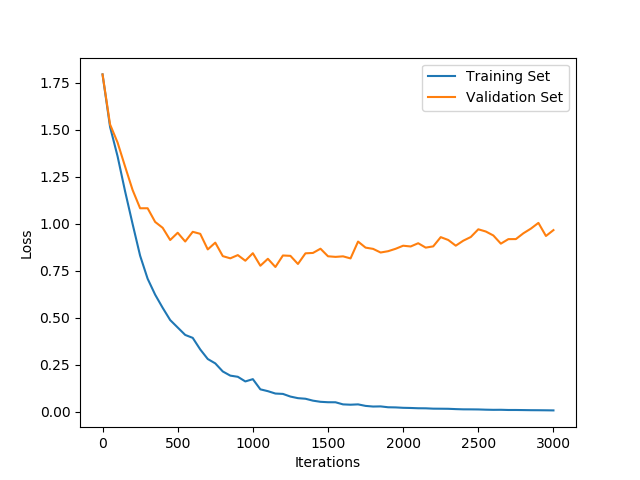
\includegraphics[width=\linewidth]{q8}
		\caption{Learning curve for the training and validation set with an image size of \(64\cross64\) pixels with a hidden layer of twenty units, initial learning rate of \num{1e-3}, batch size of 30, and using the ReLU activation function optimized over 3000 iterations.}
		\label{q8}
	\end{figure}
\end{problem}
\clearpage

%----------------------------------------------------------------------------------------
%	PART 9
%----------------------------------------------------------------------------------------

\FloatBarrier
\begin{problem}
	The visualization of the weights important for classifying an image as either Alec Baldwin or Angie Harmon are shown in \cref{q9}. The group were selected by first finding the average activation of the hidden layer across a 100 images of each person. These activations were then multiplied with the weights feeding into the output associated with each person to obtain the contribution of each hidden unit to the classification of person into a category. The percentage difference between the contribution of each hidden unit to the classification of an image as one person or the other was found, and those hidden units with the largest percentage difference were selected as the most important for the classification and are shown below.
	
	\begin{figure}
		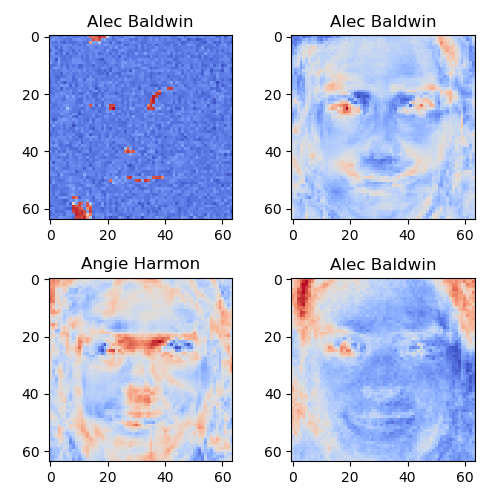
\includegraphics[width=\linewidth]{q9}
		\caption{Visualization of the weights important for classifying an image as Alec Baldwin or Angie Harmon. The title above each image denotes the actor/actress that a larger positive activation of the associated hidden unit signifies. Note the resemblance of several of the images to faces.}
		\label{q9}
	\end{figure}
	
\end{problem}
\clearpage

%----------------------------------------------------------------------------------------
%	PART 10
%----------------------------------------------------------------------------------------

\FloatBarrier
\begin{problem}
	
	The activations of the fourth convolution layer were extracted by pulling the first 9 layers out of the pretrained AlexNet implementation (corresponding to convolution layer 1 through 4) then applied onto the input. These activations were flattened, stored, and used as the input for the fully-connected neural net built on top of it. This neural network is identical in its basic structure to the neural network described in question 8, is initialised in the same way, and is fed images the same way. The images are 277 by 277 pixels and are preprocessed in the same way as in the sample provided.
	
	Based on the experience obtained in question 8, the hyper parameters were selected. These obtained exceptional performance, so it was decided that no further tuning was required. The neural net had one hundred nodes in its hidden layer and uses the LeakyReLU activation function with negative slope of 0.01. This network was trained with a batch size of one hundred units over one hundred epochs, achieving a final accuracy of 95.69\%. The learning curve is visualized in \cref{q10}. Note that the obtained activations were first detached from AlexNet so that the gradient would not be computed over them.
	
	\begin{figure}
		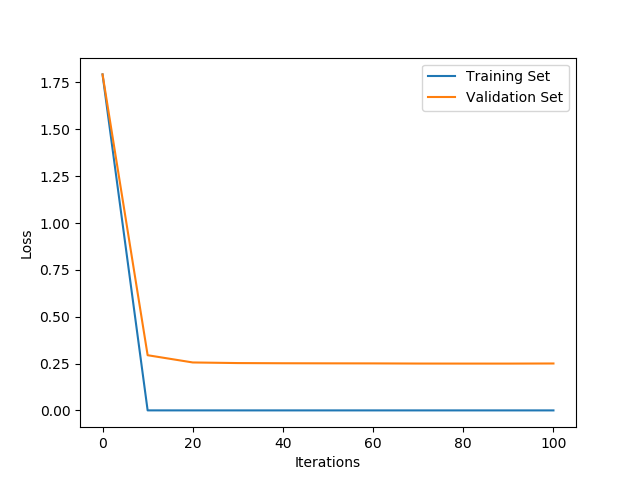
\includegraphics[width=\linewidth]{q10}
		\caption{Learning curve for fully-connected neural network built on top of the activations of the conv4 layer of AlexNet.}
		\label{q10}
	\end{figure}
	
\end{problem}
\clearpage

%----------------------------------------------------------------------------------------

\end{document}